% !TeX root = ../main.tex

\chapter{地面运行的LXeTPC本底研究}
\label{sec:backgrounds}

为了定量地描述实验对某些物理参数的灵敏度,我们需要对实验本底进行估计。
本章使用蒙特卡洛方法(Monte Carlo method),估计两类实验中的主要本底:$\mu$子本底和材料放射性本底,
以及信号筛选条件对两类本底的压低能力。

\section{模拟框架}

Geant4 是辐射探测和粒子物理领域常用的以C++为基础的蒙特卡洛模拟软件包\cite{agostinelli_geant4simulation_2003,allison_geant4_2006,allison_recent_2016}。
PandaX合作组基于Geant4开发了BambooMC软件包用于PandaX实验中的探测器模拟\cite{chen_bamboomc_2021}。
BambooMC具有较强的可拓展性,本文中使用基于BambooMC开发的软件包RelicsSim对地表附近探测器$\mu$事件和材料本底进行模拟。
所用几何如图\ref{fig:relics_g4}所示,结构遵循\ref{fig:relics_geo}的设计,
绿色体积为液氙4$\pi$反符合探测器,蓝色体积为中心主探测器。

\begin{figure}
  \begin{subfigure}{.5\textwidth}
    \centering
    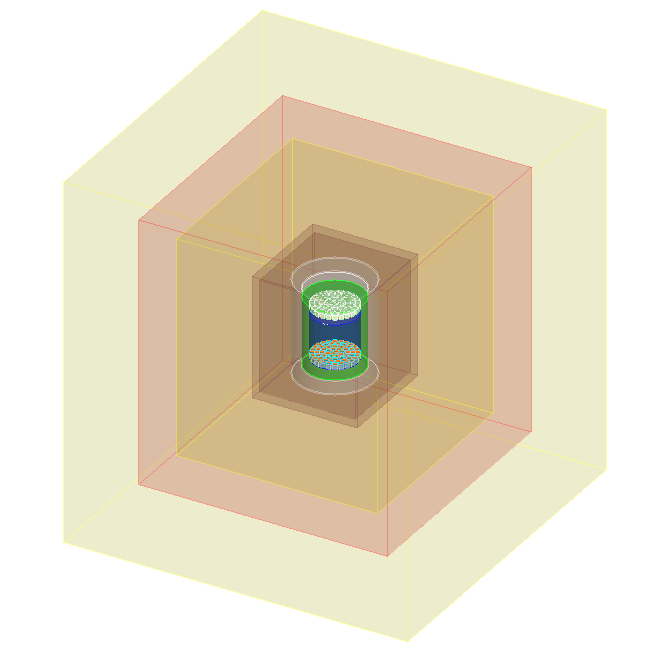
\includegraphics[width=1.0\linewidth]{figures/relics_outer.png}
    \caption{\label{fig:relics_outer} LXeTPC屏蔽体几何}
  \end{subfigure}
  \begin{subfigure}{.5\textwidth}
    \centering
    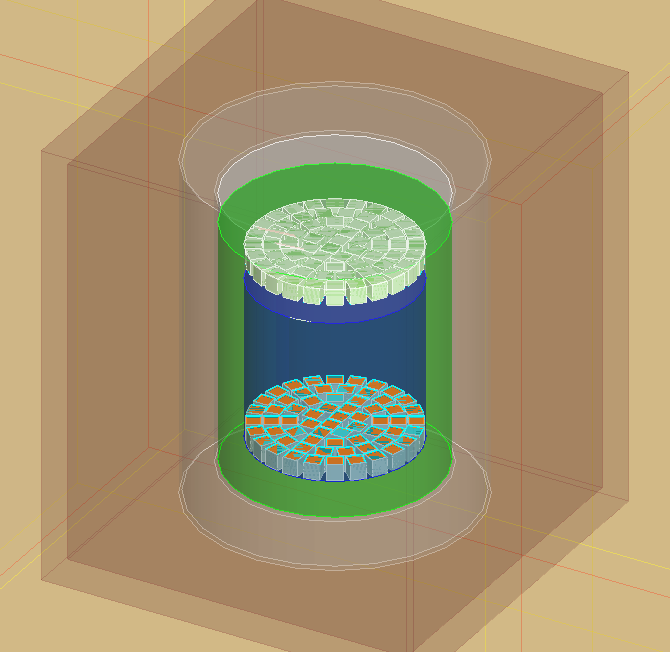
\includegraphics[width=1.0\linewidth]{figures/relics_inner.png}
    \caption{\label{fig:relics_inner} LXeTPC中心探测器几何}
  \end{subfigure}
  \caption{\label{fig:relics_g4} RelicsSim中屏蔽体和探测器几何探测器}
\end{figure}

探测器基本参数列在表\ref{tab:relics_material}中。

\begin{table}
  \centering
  \caption{LXeTPC几何参数}
  \begin{tabular}{cccc}
    \toprule
    名称 & 几何体 & 参数($\si{cm}$) & 质量($\si{kg}$) \\
    \midrule
    外聚乙烯屏蔽体 & 空心长方体 & $216\times216\times226$ & 6011.2 \\
    铅屏蔽体 & 空心长方体 & $156\times156\times166$ & 20277.3 \\
    内聚乙烯屏蔽体 & 空心长方体 & $126\times126\times136$ & 1639.2 \\
    铜屏蔽体 & 空心长方体 & $66\times66\times76$ & 640.6 \\
    空气层 & 空心长方体 & $60\times60\times70$ & - \\
    外不锈钢罐体 & 空心圆柱体 & 厚$0.5$,高$59$,直径$48$ & 49.0 \\
    真空隔热层 & 空心圆柱体 & 厚$5$,高$58$,直径$47$ & - \\
    内不锈钢罐体 & 空心圆柱体 & 厚$0.5$,高$48$,直径$37$ & 30.1 \\
    外层气态氙 & 圆柱体 & 高$5$,直径$36$ & - \\
    液氙反符合层 & 空心圆柱体 & 厚$4$,高$42$,直径$36$ & 61.3 \\
    内层气态氙 & 圆柱体 & 高$6$,直径$28$ & - \\
    液氙主探测器 & 圆柱体 & 高$28$,直径$28$ & 41.8 \\
    \bottomrule
  \end{tabular}
  \label{tab:relics_material}
\end{table}

液氙主探测器上下分别有64个1英寸光电倍增管:日本滨松R8520,共128个。光电倍增管的几何如图\ref{fig:pmt_geo},
蓝色透明几何为石英窗;橙色几何为光阴极(photocathode);灰色部分是外壳(casing),材质为SAE 304不锈钢。
设计的PMT排布保证了轴向对称性,可能对未来的位置重建有利。

\begin{figure}
  \begin{subfigure}{.53\textwidth}
    \centering
    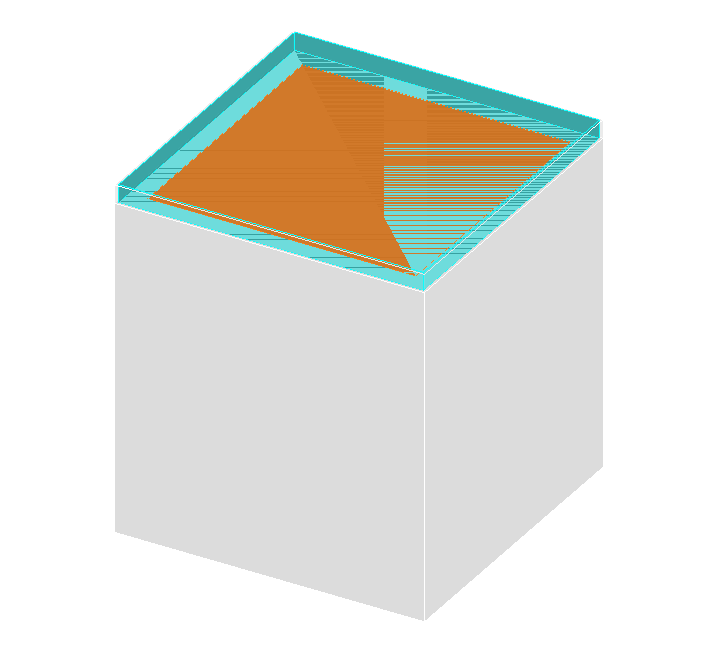
\includegraphics[width=1.0\linewidth]{figures/pmt_geo.png}
    \caption{\label{fig:pmt_g4} R8520在Geant4中的几何}
  \end{subfigure}
  \begin{subfigure}{.47\textwidth}
    \centering
    \includesvg[width=1.0\linewidth]{figures/topPMTs.svg}
    \caption{\label{fig:pmt_layout} PMT在探测器$(x,y)$平面上的排布}
  \end{subfigure}
  \caption{\label{fig:pmt_geo} 光电倍增管R8520的几何和在探测器$(x,y)$平面上的排布}
\end{figure}

PMT石英窗上富集的${}^{40}\mathrm{K}$和${}^{137}\mathrm{Cs}$可能成为主要的本底来源,具体内容将在第\ref{sec:pmt_background}章中讨论。

\section{本底事件的筛选与压低}

本底事件经常与信号有不同的性质以及测量结果。
我们可以通过选取某些具有区分能力(discrimination power)的性质,在其值域中定义选取信号并进行物理分析的区间,
在尽可能少地损失信号的条件下,去除尽可能多的本底。

对于$\mu$子本底,其可能强烈地在液氙反符合层中沉积能量,可以用反符合层对$\mu$子的标记将其本底压低。
考虑到一个物理事件的时间窗约为$200\mu s$,$\mu$子和中子将可能有足够多的时间在主探测器中多次沉积能量,
而中微子几乎只可能与探测器发生单次散射(single scatter, SS),
所以我们可以通过筛选并去除一个事件窗内有多次散射(multiple scatter, MS)的事件,对这类本底进行压低。
最后,若一个主探测器中的核反冲事件同时伴随着一个主探测器中的电子反冲事件,则这个核反冲事件有较大可能是$\mu$子引起的而不是中微子。

材料的$\beta$和$\gamma$放射性在中心探测器边缘单位体积沉积的能量比探测器中心多,所以一定程度地舍弃某些本底过高的区域,
对物理信号的搜索是有利的,选取的本底较低的区域定义为灵敏体积(fiducial volume)。
同时材料本底,有一定概率产生多次散射,如$\gamma$的康普顿散射事件,也可以通过判断是否有多次散射来去除这类本底。

所有与能量相关的筛选条件(或阈值)均需要通过详尽严格的信号模拟来确定;
灵敏体积的选取和设置也需要综合考虑物理信号和本底的空间分布。本文仅根据经验,设置粗略的信号筛选条件,
考察在这些条件下信号和本底的事例率以及相应的实验灵敏度。
针对核反冲本底和电子反冲本底,信号筛选条件列于表\ref{tab:cuts},只有满足表中所有条件的事件才被纳入物理分析。

\begin{table}
  \centering
  \caption{针对核反冲和电子反冲本底的信号筛选条件}
  \begin{tabular}{cc}
    \toprule
    名称 & 条件 \\
    \midrule
    液氙反符合(LXe veto) & 反符合层中最大的电子(核)反冲不大于$100$($500$)$\si{keV}$ \\
    NR单次散射(ER SS cut) & 主探测器中第二大的NR能量不大于最大NR能量的5\% \\
    ER单次散射(NR SS cut) & 主探测器中第二大的ER能量不大于$1\si{keV}$ \\
    NR的ER标记(ER tagging) & 主探测器中与NR事件同时发生的ER不大于$10\si{keV}$ \\
    灵敏体积(FV cut) & 气液交界面以下$0.5\si{cm}$到$24.5\si{cm}$,半径$12\si{cm}$的圆柱 \\
    \bottomrule
  \end{tabular}
  \label{tab:cuts}
\end{table}

反符合层中没有漂移电场,只有光信号,我们将在反符合层中设置PMT来探测这他们。
由于核反冲信号的淬灭效应,相同能量的核反冲和电子反冲产生的光子数不同,取淬灭因子(quenching factor)为0.2,
则将反符合层的核反冲阈值设置为电子反冲的$1/0.2=5$倍。

灵敏体积为高$24\si{cm}$,半径为$12\si{cm}$的圆柱,其中液氙总质量约为$30.5\si{kg}$。在S2-Only分析中,不引入$\mathrm{S1}$,
事件将没有电子漂移距离$z$信息,但我们让然可以通过$\mathrm{S2}$波形的事件分布一定程度上判断事件发生的纵向位置,
所以这里对S2-Only和S1-S2分析设置了相同的灵敏体积。

\section{$\mu$子本底}

地面附近运行的LXeTPC将会经受原生宇宙线和次生宇宙线的轰击。
来自外部空间的宇宙线成分以高能质子为主,在穿越地球大气层的过程中与大气分子发生簇射反应,产生大量次级粒子,
主要包括质子、$\mu$子、电子、中子、$\gamma$光子等。宇宙线粒子通量与大气层深度有关,如图\ref{fig:vertical_flux},
$\mu$子和中微子是地面附近通量最高的两种粒子,中微子较少与物质发生相互作用,$\mu$子成为实验中的主要本底。

\begin{figure}
    \centering
    \includesvg[width=0.6\linewidth]{figures/vertical_flux.svg}
    \caption{\label{fig:vertical_flux} 宇宙线中不同粒子通量与大气深度的关系\cite{olive_review_2016}}
\end{figure}

$\mu$子是带电粒子,穿透能力较强。$\mu$子穿越物质的过程中通过电磁相互作用减速,产生电离,
高能($10\si{GeV}$以上)$\mu$子在物质中的能损$-\mathrm{d}E/\mathrm{d}x$大约为$2\si{MeV\cdot cm^{-1}}$。
考虑相对论时间膨胀效应,$\mu$子在物质中能够穿越较长距离。$\mu$子还有可能被原子核俘获,
使靶原子核序数减1,同时放出1个或多个中子。这些中子将是探测器中核反冲本底的主要来源。

利用$\mu$子持续产生电离的特点,可以在探测器外围部署$\mu$子反符合探测器,
当$\mu$子同时在反符合探测器和主探测器产生信号且符合一定条件时时,通过硬件触发或软件筛选,
可以将主探测器中事件标记为$\mu$子事件以区分信号的本底。但物理信号如CE$\nu$NS也有一定几率发生在$\mu$子穿越探测器时,
这时对$\mu$子事件的标记会使物理信号的探测效率降低,等效为曝光量(exposure)的损失,这种效应必须考虑到统计推断中,
否则将高估探测器中产生的信号。

地面附近的$\mu$子分布可以用Gaisser公式或Shukla公式描述。T.K.Gaisser在忽略地球曲率的情况下,
给出了$\mu$子通量随$\mu$子能量$E_\mu$和天顶角(zenith angle)$\theta$的分布。天顶角为入射粒子与地面法线间的夹角\cite{gaisser_cosmic_2016}。

\begin{align}
    \label{eq:gaisser}
    \frac{\mathrm{d}N_\mu}{\mathrm{d}E_\mu\mathrm{d}\Omega} &\approx 
    1400E_\mu^{-2.7}/\left(\si{m^2\cdot s\cdot GeV\cdot sr}\right)\left(\frac{1}{1+\frac{1.1E_\mu\cos\theta}{\epsilon_\pi}}+\frac{0.054}{1+\frac{1.1E_\mu\cos\theta}{\epsilon_\kappa}}\right)
\end{align}

其中$\epsilon_\pi\approx115\si{GeV},\epsilon_\kappa\approx850\si{GeV}$。
Gaisser公式只在高能区间($E_\mu>(100/\cos\theta)\si{GeV}$)适用。

P.Shukla等人在考虑地球曲率的条件下给出了类似的分布\cite{shukla_energy_2018},如式\ref{eq:shukla}:

\begin{align}
    \label{eq:shukla}
    I\left(E_\mu,\theta\right) &= I_0 N\left(E_0+E_\nu\right)^{-n}\left(1 + \frac{E_\mu}{\epsilon_\mu}\right)^{-1}D(\theta)^{-(n-1)} \\
    D(\theta) &= \sqrt{\frac{R^2}{d^2}\cos^2\theta+2\frac{R}{d}+1}-\frac{R}{d}\cos\theta
\end{align}

其中$I_0$为绝对流强,$N$为归一化参数,$n$为天顶角分布的幂次,$\epsilon_\mu,\frac{R}{d}$为经验公式中的自由参数。
使用不同地点测量得到的$\mu$子分布可以拟合得到不同结果,这里我们使用通过日本筑波市附近的测量数据得到的拟合结果,具体参数见表\ref{tab:shukla}。
Shukla公式在低能区域和高能区域都与数据符合得较好。

\begin{table}
  \centering
  \caption{描述$\mu$子分布的Shukla公式采用的参数列表}
  \begin{tabular}{cc}
    \toprule
    符号 & 取值 \\
    \midrule
    $I_0$ & $70.7\si{m^{-2}\cdot s^{-1}\cdot sr^{-1}}$ \\
    $n$ & 3.01 \\
    $E_0$ & $4.19\si{GeV}$ \\
    $\epsilon_\mu$ & $854\si{GeV}$ \\
    $R/d$ & $174$ \\
    \bottomrule
  \end{tabular}
  \label{tab:shukla}
\end{table}

式\ref{eq:shukla}中天顶角$\theta$相关的项可以从$E_\mu$中解耦合,$\theta$和$E_\mu$的分布如图\ref{fig:shukla_distribution},
$\theta$主要集中在夹角较小的区域,
因为天顶角更大的$\mu$子与大气层中物质的相互作用路程更长,损失更多;$E_\mu$的分布主要集中在低能部分。

\begin{figure}
    \centering
    \includesvg[width=0.8\linewidth]{figures/shukla_distribution.svg}
    \caption{\label{fig:shukla_distribution} Shukla公式中$\theta$和$E_\mu$的分布}
\end{figure}

对Shukla公式进行积分,可以得到海平面附近全能谱$\mu$子通量约为$150\si{m^{-2}\cdot s^{-1}}$。

到达地面附近的$\mu$子包含了$\mu^-$和$\mu^+$。
CMS于2010年测量了地表附近的$\mu$子电荷比(charge ratio, $I_{\mu^+}/I_{\mu^-}$)约为$1.2766\pm0.0045$\cite{the_cms_collaboration_measurement_2010}。
$\mu$子电荷比在$\mu$子动量小于$100\si{GeV/c}$时与能量几乎无关,且在更高动量的区域略增大。
考虑到第\ref{sec:muon_nr}节中讨论的$\mu$子核反冲本底主要由较低能量的$\mu^-$贡献,更高的电荷比意味着更低的核反冲本底,本文保守地使用不随能量变化的电荷比。

模拟中将从屏蔽体外部一个足够的水平平面上均匀取点作为$\mu$子的入射位置,通过Shukla公式对$\mu$子的入射角和能量进行采样,
模拟几何如图\ref{fig:muon_inject},最顶部平面为$\mu$子初始位置,蓝色圆柱体为液氙探测器。

\begin{figure}
  \centering
  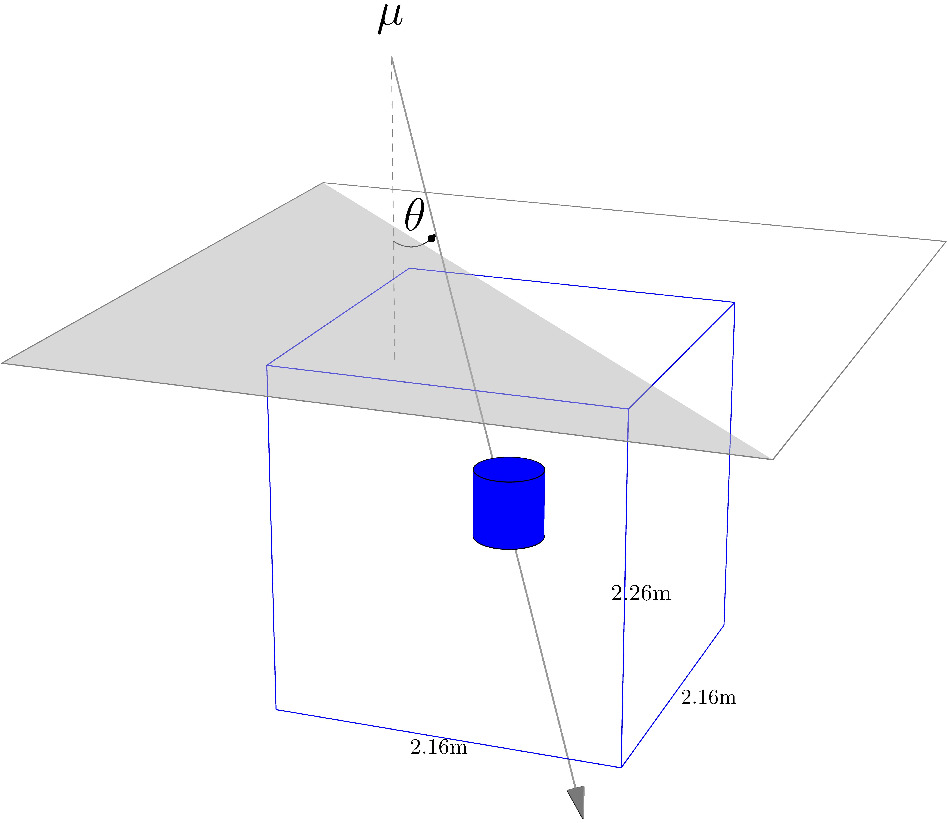
\includegraphics[width=0.6\linewidth]{figures/muon_inject.pdf}
  \caption{\label{fig:muon_inject} 模拟$\mu$子入射屏蔽体和探测器的示意图}
\end{figure}

Geant4模拟中设置中心探测器和液氙反符合屏蔽层为灵敏探测器,并记录两种灵敏探测器中的能量沉积。
因液氙中相近时间且相近空间位置的能量沉积并不能被有效区分,
得到模拟结果后将使用聚类算法DBSCAN(Density-Based Spatial Clustering of Applications with Noise)\cite{ester_density-based_1996,schubert_dbscan_2017}合并临近时空中的能量沉积。

本文中假设$\mu$子反符合探测器的探测效率为99\%,且不随$\mu$子能量变化,
即假设只有1\%的$\mu$子事件的能量沉积不能被$\mu$子反符合探测器标记并最终形成被记录的本底。

\subsection{核反冲本底}
\label{sec:muon_nr}

$\mu$子主要通过两种方式产生核反冲。高能$\mu$子可以直接与原子核发生库伦散射使原子核获得动能;
低能$\mu$子有跟高的概率被原子核俘获,之后放出一个或几个中子。图\ref{fig:muon_nr}列出了$\mu$子引起核反冲的总能谱,
其中按顺序施加了灵敏体积、液氙反符合、对核反冲的电子反冲标记、核反冲单次散射等筛选条件。

\begin{figure}
  \centering
  \includesvg[width=0.9\linewidth]{figures/muon_nr.svg}
  \caption{\label{fig:muon_nr} $\mu$子引起的核反冲能谱}
\end{figure}

液氙反符合对$\mu$子核反冲的压低能力在我们关心的能区$[0.1,1]\si{keV}$最强,
因为低能中子产生多次散射的概率不高,NR SS cut的压低能力并不显著,图中只有高能部分的NR被其显著压低。
在施加筛选条件之后,$[0.1,1]\si{keV}$中的事例率为$0.30\left(\si{kg}\cdot\si{day}\right)^{-1}$,
空间分布如图\ref{fig:muon_nr_xyzr},能量沉积略集中在探测器边缘。

\begin{figure}
  \centering
  \includesvg[width=1.0\linewidth]{figures/muon_nr_xyzr.svg}
  \caption{\label{fig:muon_nr_xyzr} $\mu$子引起的核反冲经过筛选条件压低后的空间分布}
\end{figure}

\subsection{电子反冲本底}

$\mu$子带电,$\mu$子事件的电子反冲本底主要由$\mu$子在物质中的直接电离引起。如图\ref{fig:muon_er},
其中左图为全区能谱,右图为$[0, 100]\si{keV}$能区能谱,
其中按顺序施加了灵敏体积、液氙反符合、电子反冲单次散射等筛选条件。

\begin{figure}
  \centering
  \includesvg[width=1.0\linewidth]{figures/muon_er.svg}
  \caption{\label{fig:muon_er} $\mu$子引起的电子反冲能谱}
\end{figure}

对于高能$\mu$致电子反冲,液氙反符合的效果非常明显,在施加该条件后,几乎所有$5\si{MeV}$以上的电子反冲事件都会被排除。
要求电子反冲单次散射也会将本底压低近1个量级。
\ref{fig:muon_er}右图能谱的形状可能是低能区域模拟事件统计量的涨落所致,也可能是$\mu$子对物质原子核激发产生的特征$\gamma$射线的能谱,具体原因有待考察。

$[0, 100]\si{keV}$能区$\mu$子引起的电子反冲的空间分布在探测器上部分布略集中,如图\ref{fig:muon_er_xyzr}。

\begin{figure}
  \centering
  \includesvg[width=1.0\linewidth]{figures/muon_er_xyzr.svg}
  \caption{\label{fig:muon_er_xyzr} $\mu$子引起的电子反冲经过筛选条件压低后的空间分布}
\end{figure}

表\ref{tab:cuts_muon_remain}列出了几种筛选条件后的$\mu$子核反冲在$[0.1,1]\si{keV}$能区和电子反冲在的$[0,100]\si{keV}$能区剩余事例率,误差棒来自模拟事例个数的统计误差。

\begin{table}
  \centering
  \caption{$\mu$子引起的$[0.1,1]\si{keV}$内核反冲和$[0,100]\si{keV}$内电子反冲的本底剩余事例率}
  \begin{tabular}{ccc}
    \toprule
    筛选条件 & NR事例率$\left(10^{-2}\left(\si{kg}\cdot\si{day}\right)^{-1}\right)$ & ER事例率$\left(10^{-3}\left(\si{kg}\cdot\si{keV}\cdot\si{day}\right)^{-1}\right)$ \\
    \midrule
    无筛选条件 & $115.2_{-1.3}^{+1.3}$ & $36.0_{-0.2}^{+0.2}$ \\
    灵敏体积(FV cut) & $93.5_{-1.4}^{+1.4}$ & $14.2_{-0.2}^{+0.2}$ \\
    液氙反符合(LXe veto) & $30.4_{-0.8}^{+0.8}$ & $7.4_{-0.1}^{+0.1}$ \\
    NR的ER标记(ER tagging) & $23.5_{-0.7}^{+0.7}$ & - \\
    NR单次散射(NR SS cut) & $23.5_{-0.7}^{+0.7}$ & - \\
    ER单次散射(ER SS cut) & - & $4.9_{-0.1}^{+0.1}$ \\
    \bottomrule
  \end{tabular}
  \label{tab:cuts_muon_remain}
\end{table}

\section{材料本底}

相比于$\mu$子本底,材料本底是地面实验和地下实验都需要处理的本底。
材料本底主要来自屏蔽体、罐体、光电倍增管、整形环、聚四氟乙烯反射板、以及液氙等。
本文主要模拟来自屏蔽体、光电倍增管和液氙的放射性本底。

因一半放射性同位素含量与材料有关而与材料所处空间位置基本无关,BambooMC设计了\verb|Confine Generator|用于模拟某种材料放射性。
其工作原理如下:首先指定需要进行模拟的材料,然后随机在足够大的空间中均匀采样,通过设计的几何关系判断采样点对应的几何体的材料是否为预先指定的,
若是,则放置放射性核素的原子(或离子);若不是,则继续在空间中撒点直到选取到指定的材料为止。这种模拟方式不需要精确描述放射源的初始位置,较简便,
同时也默认了所有材料放射源在材料中均匀分布。

屏蔽体和罐体的材料主要为金属。金属矿石与长半衰期的原生放射性核素共生,
如${}^{238}\mathrm{U},{}^{232}\mathrm{Th},{}^{40}\mathrm{K}$等。
PMT石英窗(主要成分为$\mathrm{Si}\mathrm{O}_2$)因为$\mathrm{Si}$与碱金属元素的亲和性,也含有一定量的${}^{40}\mathrm{K}$。
这些核素的半衰期非常长,如${}^{238}\mathrm{U}$的半衰期为45亿年。
如此长的半衰期使得,在矿石中这些核素与其衰变链上的子核将建立长期平衡(secular equilibrium),具体表现为母核核素与子核核素的放射性活度相等。
这对我们计算核素长衰变链上的放射性活度提供了便利。
然而事实上对矿石的开采冶炼和一些其他过程可能会破坏长期平衡,导致母核与子核核素的活度不等,此时为了估计材料放射性,就需要对进行实地测量,
并以实地测量的结果作为蒙特卡洛的输入量。本文中假定长期平衡不被破坏,即将长半衰期核素的活度作为全衰变链上子核的活度,
如认为${}^{238}\mathrm{U}$与其链上的${}^{226}\mathrm{Ra}$活度相等。

金属中还可能含有${}^{60}\mathrm{Co}$等人工放射性核素和${}^{3}\mathrm{H}$等宇生放射性核素,在模拟中也将一并考虑。

BambooMC提供了\verb|DecayChainSplitting|功能用于模拟衰变链上的核素。考虑到探测器的时间窗约为$200\mu s$,
则衰变链上的较长半衰期核素如${}^{226}\mathrm{Ra}$($T_{1/2}=1602y$)几乎可能与其母核在同一个时间窗内衰变。在模拟中,我们可以将衰变链通过判断核素半衰期长度的方式分解。
首先设置一个阈值,如$200\mu s$,对于任何半衰期长于阈值的核素,我们都将其作为一个新的模拟事件的母核对待,
同时新事件的时间也会归零,这样很大程度上与实际情况是符合的。这种操作减少了遍历每一种衰变链上核素的工作量。

\subsection{光电倍增管本底}
\label{sec:pmt_background}

光电倍增管(PMT)上的本底主要有石英窗上的${}^{40}\mathrm{K},{}^{137}\mathrm{Cs},{}^{238}\mathrm{U}$和金属外壳上的${}^{238}\mathrm{U},{}^{232}\mathrm{Th}$等,即这些核素的子核。
模拟中的PMT结构见图\ref{fig:pmt_geo}。放射性核素的具体含量见表\ref{tab:pmt_radio},数据来自XENON100的电子反冲本底研究\cite{xenon100_collaboration_study_2013}。

\begin{table}
  \centering
  \caption{PMT上每部分结构放射性同位素比活度,单位均为$\si{mBq\cdot kg^{-1}}$}
  \begin{tabular}{ccc}
    \toprule
    核素 & PMT石英窗 & PMT外壳 \\
    \midrule
    ${}^{238}\mathrm{U}$ & 0.14 & 0.16 \\
    ${}^{232}\mathrm{Th}$ & 0.17 & 0.07 \\
    ${}^{60}\mathrm{Co}$ & 0.62 & 0.01 \\
    ${}^{40}\mathrm{K}$ & 11.1 & 0.16 \\
    ${}^{137}\mathrm{Cs}$ & 0.79 & 0 \\
    \bottomrule
  \end{tabular}
  \label{tab:pmt_radio}
\end{table}

模拟中PMT的石英窗质量为$2\si{g}$,外壳质量为$13.6\si{g}$。

\subsection{屏蔽体材料本底}

屏蔽体和罐体材料中的本底含量如表\ref{tab:shield_radio}。

\begin{table}
  \centering
  \caption{屏蔽体和罐体组件中放射性同位素比活度,单位均为$\si{mBq\cdot kg^{-1}}$}
  \begin{tabular}{ccccc}
    \toprule
    核素 & 聚乙烯屏蔽层 & 铅屏蔽层 & 铜屏蔽层 & 不锈钢罐体 \\
    \midrule
    ${}^{238}\mathrm{U}$ & 0.23 & 0.92 & 0.08 & 1.8 \\
    ${}^{232}\mathrm{Th}$ & 0.09 & 0.72 & 0.01 & 1.9 \\
    ${}^{60}\mathrm{Co}$ & 0 & 0.12 & 0.04 & 5.4 \\
    ${}^{40}\mathrm{K}$ & 0.68 & 0.01 & 0.03 & 9 \\
    ${}^{210}\mathrm{Pb}$ & 0 & $5.14\times10^5$ & 0 & 0 \\
    \bottomrule
  \end{tabular}
  \label{tab:shield_radio}
\end{table}

\subsection{液氙中惰性元素本底}

本文中主要考虑的液氙中惰性元素本底为${}^{222}\mathrm{Rn}$和${}^{85}\mathrm{Kr}$。

${}^{222}\mathrm{Rn}$在${}^{238}\mathrm{U}$的衰变链中产生,探测器材料会持续放出${}^{222}\mathrm{Rn}$。
考虑到${}^{222}\mathrm{Rn}$半衰期为$3.8d$,其和其子核将在液氙体积中均匀地衰变\cite{the_xenon_collaboration_projected_2020}。
本文中假定其比活度为$40\mu\si{Bq\cdot kg^{-1}}$。
${}^{222}\mathrm{Rn}$衰变链上的${}^{210}\mathrm{Pb}$半衰期为$22.4y$,相比于探测器运行时间,
${}^{210}\mathrm{Pb}$对放射性的贡献可以忽略,其后续所有衰变的放射性也将不考虑到模拟结果中。

自然界的$\mathrm{Kr}$元素中含有痕量的${}^{85}\mathrm{Kr}$(半衰期$T_{1/2}=10.76y$)。
其$\beta$衰变能谱中最大能量为$685\si{keV}$,使其在低能分析中,成为不可忽略的重要本底。
${}^{85}\mathrm{Kr}$的丰度为${}^{85}\mathrm{Kr}/{}^\mathrm{nat}\mathrm{Kr}=(1.7\pm0.3)\times 10^{-11}$\cite{the_xenon_collaboration_projected_2020}。
本文中假定${}^\mathrm{nat}\mathrm{Kr}$在液氙中的含量为$10\mathrm{ppt}{}^\mathrm{nat}\mathrm{Kr}/\mathrm{Xe}$,且${}^{85}\mathrm{Kr}$活度不随着时间变化($1\mathrm{ppt}=10^{-12}$)。

将所有材料放射性的电子反冲本底叠加,得到汇总,如图\ref{fig:muon_er},其中左图为全区能谱,
右图为$[0, 100]\si{keV}$能区能谱,其中按顺序施加了灵敏体积、液氙反符合、电子反冲单次散射等筛选条件。

\begin{figure}
  \centering
  \includesvg[width=1.0\linewidth]{figures/material_er.svg}
  \caption{\label{fig:material_er} 材料放射性电子反冲本底汇总}
\end{figure}

灵敏体积 cut 对电子反冲本底的压低效果很强,这主要是因为$\mathrm{Xe}$的辐射屏蔽效果很强,PMT放射性大多集中在TPC的阴极以下及液氙上表面;
且不锈钢罐体的主要放射性集中靠近罐体的区域。电子反冲单词散射对较高能的本底压低效果很强,因为几百$\si{keV}$的$\gamma$光子更容易产生多次散射效应。

低能区域($[0, 100]\si{keV}$)的能谱较平坦,在施加筛选条件后主要剩余本底来自于${}^{85}\mathrm{Kr}$和PMT,${}^{222}\mathrm{Rn}$的贡献在$1\times10^{-3}\si{kg}\cdot\si{keV}\cdot\si{day}$以下。

材料放射性电子反冲本底经过筛选条件压低后的空间分布略集中在灵敏体积边缘,如图\ref{fig:material_er_xyzr}。

\begin{figure}
  \centering
  \includesvg[width=1.0\linewidth]{figures/material_er_xyzr.svg}
  \caption{\label{fig:material_er_xyzr} 材料放射性电子反冲本底经过筛选条件压低后的空间分布}
\end{figure}

表\ref{tab:cuts_material_remain}列出了几种筛选条件后的材料放射性电子反冲本底在$[0,100]\si{keV}$能区剩余事例率,误差棒来自模拟事例个数的统计误差。

\begin{table}
  \centering
  \caption{材料放射性中$[0,100]\si{keV}$内电子反冲的本底剩余事例率}
  \begin{tabular}{ccc}
    \toprule
    筛选条件 & 事例率$\left(10^{-3}\left(\si{kg}\cdot\si{keV}\cdot\si{day}\right)^{-1}\right)$ \\
    \midrule
    无筛选条件 & $1808.6_{-4.1}^{+4.1}$ \\
    灵敏体积(FV cut) & $62.6_{-0.5}^{+0.5}$ \\
    液氙反符合(LXe veto) & $20.8_{-0.2}^{+0.2}$ \\
    ER单次散射(ER SS cut) & $14.3_{-0.1}^{+0.1}$ \\
    \bottomrule
  \end{tabular}
  \label{tab:cuts_material_remain}
\end{table}

图\ref{fig:all_event_rate}是两种本底和信号的汇总,因核反冲信号的淬灭效应,取淬灭因子为0.2,
将核反冲能量$T_\mathrm{nr}$乘淬灭因子转化后与电子反冲能量进行比较。

\begin{figure}
  \centering
  \includesvg[width=0.7\linewidth]{figures/all_event_rate.svg}
  \caption{\label{fig:all_event_rate} $\mu$子与材料的本底汇总,蓝色阴影为进行物理搜索的主要能区}
\end{figure}

根据\ref{sec:lxe_signal}节中的LXeTPC响应,信号和本底的$\mathrm{S2}$电子谱为图\ref{fig:S2e_rate_bkg},
将使用4-10个电子的区域进行物理搜索。

\begin{figure}
  \centering
  \includesvg[width=0.7\linewidth]{figures/S2e_rate_bkg.svg}
  \caption{\label{fig:S2e_rate_bkg} $\mu$子与材料的本底电子谱}
\end{figure}
